\documentclass{jsarticle}
\usepackage[dvipdfmx]{graphicx}
\usepackage{listings}
\usepackage{afterpage}
\begin{document}
\title{課題7 ダイナミックレンジの拡大}
\author{13EC060 武澤 裕介}
\maketitle
\begin{abstract}
matlabを用いて、ダイナミックレンジの拡大を行い、考察する。
\end{abstract}
\section{画像のヒストグラム}
まず、今回使用する原画像を図1に示す。


\begin{figure}[htbp]
 \begin{center}
  
\includegraphics[width=5cm,height=5cm]{sample.jpg}
 \end{center}
 \caption{原画像}
\end{figure}

\begin{lstlisting}[basicstyle=\ttfamily\footnotesize, frame=single]
filename = uigetfile('*');
ORG=imread(filename); % 原画像の入力
ORG = rgb2gray(ORG); colormap(gray); colorbar;
imagesc(ORG); axis image; % 画像の表示
pause; % 一時停止
 \end{lstlisting}
を用いてまず入力画像のグレースケール画像を表示させる。

\newpage
\begin{figure}[htbp]
 \begin{center}
  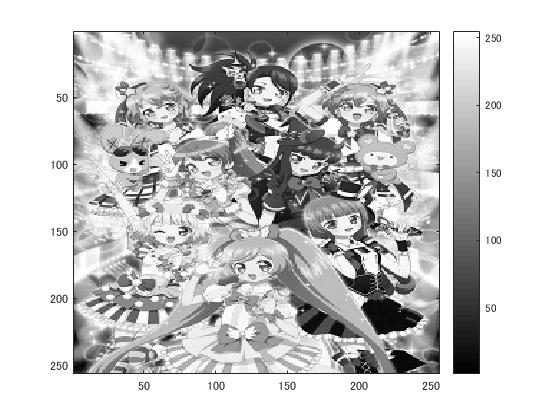
\includegraphics[width=10cm]{kadai7-0.jpg}
 \end{center}
 \caption{グレースケール画像}
\end{figure}

次に
\begin{lstlisting}[basicstyle=\ttfamily\footnotesize, frame=single]
imhist(ORG); % ヒストグラムの表示
 \end{lstlisting}
を用いて画像の輝度ヒストグラムを表示する。

\newpage
\begin{figure}[htbp]
 \begin{center}
  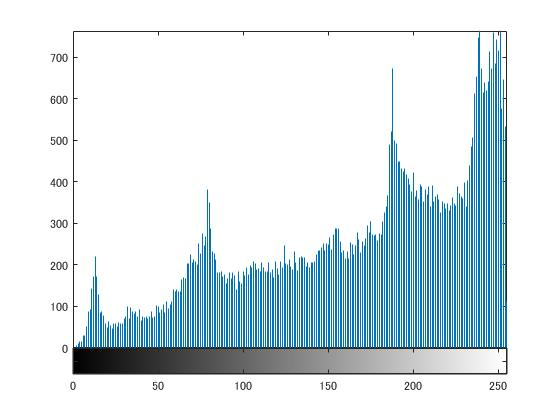
\includegraphics[width=10cm]{kadai7-1.jpg}
 \end{center}
 \caption{輝度ヒストグラム(グレースケール画像)}
\end{figure}

\begin{lstlisting}[basicstyle=\ttfamily\footnotesize, frame=single]
ORG = double(ORG);
mn = min(ORG(:)); % 濃度値の最小値を算出
mx = max(ORG(:)); % 濃度値の最大値を算出
ORG = (ORG-mn)/(mx-mn)*255;
imagesc(ORG); colormap(gray); colorbar; % 画像の表示
pause;
ORG = uint8(ORG); % この行について考察せよ
imhist(ORG); % 濃度ヒストグラムを生成、表示
 \end{lstlisting}
を用いてダイナミックレンジの拡大を行い、また濃度ヒストグラムの生成を行う。
\newpage
\begin{figure}[htbp]
 \begin{center}
  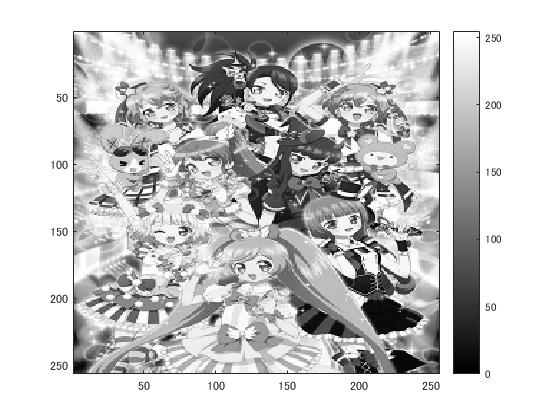
\includegraphics[width=10cm]{kadai7-2.jpg}
 \end{center}
 \caption{ダイナミックレンジの拡大後}
\end{figure}

\newpage
\begin{figure}[htbp]
 \begin{center}
  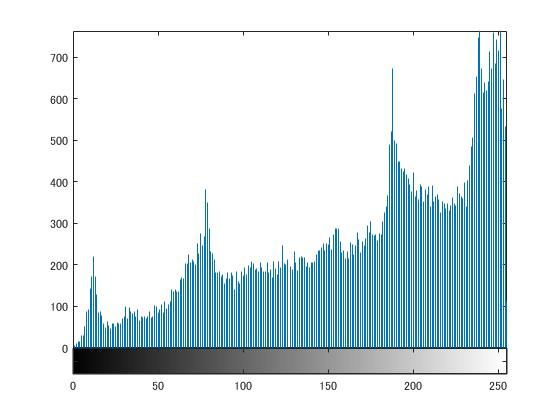
\includegraphics[width=10cm]{kadai7-3.jpg}
 \end{center}
 \caption{輝度ヒストグラム(ダイナミックレンジの拡大後)}
\end{figure}

\section{考察}
まず、図2と図4を比べるとダイナミックレンジの拡大後の画像の方が色合いが少し豊かに見えている事が分かる。また、図3と図5を比べるとダイナミックレンジの拡大後の方が濃度が0付近の部分を見ると分かるがヒストグラムの分布が広がっている事がわかる。またなぜuint8型にしているのかというとdouble型のままでヒストグラムを作ると、濃度値の刻み幅が細かすぎてヒストグラムの頻度に偏りがなくみえてしまうためである。

\end{document}